\documentclass[10pt]{article}
\linespread{1.03}% 6 lpi http://tex.stackexchange.com/questions/23824/6-lines-in-one-inch
\usepackage{mathpazo, url, amsmath, amsfonts, amssymb, mdwlist, graphicx, xcolor, stackrel, mdframed, enumitem}
\usepackage{tikz}
\usepackage[top=0.8in,bottom=0.8in,left=1in,right=1in]{geometry}
\usepackage[none]{hyphenat} \raggedright \parskip4pt  \parindent0pt
\usepackage{caption} \captionsetup{width=0.8\textwidth}
\usepackage{array}
\newcolumntype{L}[1]{>{\raggedright\let\newline\\\arraybackslash\hspace{0pt}}p{#1}}
\newcolumntype{C}[1]{>{\centering\let\newline\\\arraybackslash\hspace{0pt}}p{#1}}
\newcolumntype{R}[1]{>{\raggedleft\let\newline\\\arraybackslash\hspace{0pt}}p{#1}}
\renewcommand{\arraystretch}{1.3}

%%%%%
\begin{document}


\vspace*{-0.6in}
\begin{flushright}
\begin{tabular}{|R{2in}|} \hline 
Name: \underline{\hspace*{1.5in}}  \\ 
Date: \underline{\hspace*{1.5in}} \\ \hline
\end{tabular}
\end{flushright}

\vspace*{-0.8in}
\section*{Algebraic Knowledge for Secondary Teaching}

%1. how the definition of graph of function can be used to understand graphs of functions obtained by combining existing functions (e.g., using composition, addition, multiplication).

\begin{enumerate}
\item % Carlies item 
$\;$ \\ 

\vspace*{-8.5pt}
\begin{minipage}{3.5in}\raggedright \parskip4pt
During a lesson in your Algebra I class, suppose that you ask your students to find a quadratic function that corresponds to the graph and table shown, and to explain how they determined their answers.  
 

One student explains: ``I got $f(x)=x^2-1$. I graphed $y=x^2$ on my graphing calculator and I saw that if I translated it down 1 unit it would line up with the graph and table values.''
\end{minipage}
\begin{minipage}{2.6in}
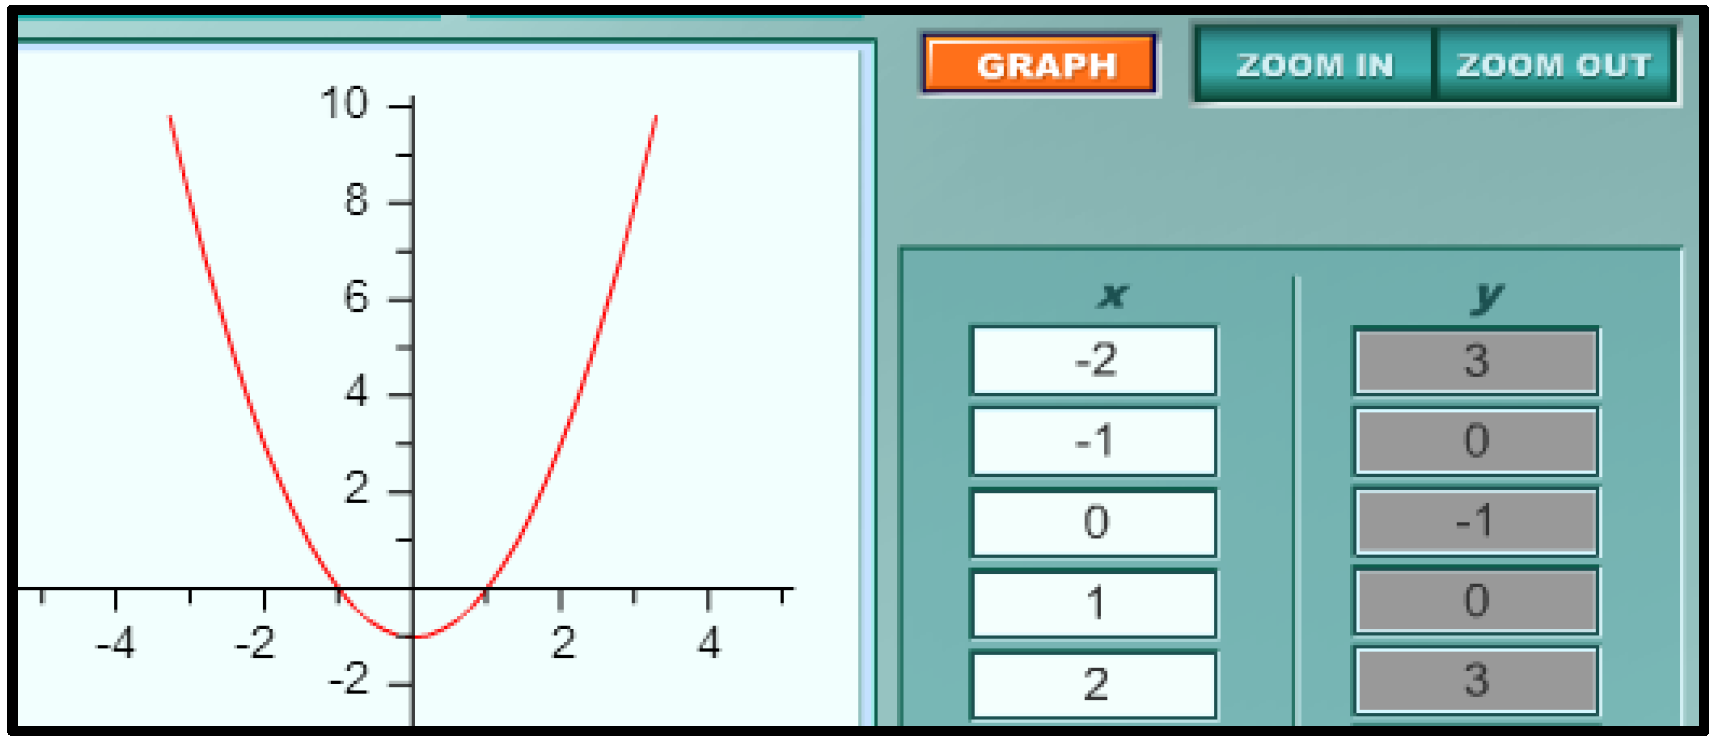
\includegraphics[width=2.5in]{Carlies_Graphic.png}
\end{minipage}

	
	\begin{enumerate}
	\item What is worthwhile about the student's thinking? List some features.
	\end{enumerate}
	
		\vspace*{-12pt}\begin{mdframed} \vspace*{1.75in} \end{mdframed}
		
	\vspace*{-12pt}
	\begin{enumerate}[resume]
	\item What would you say to help the student complete their thinking (if there are gaps in the thinking), prompt the student to investigate an error, or help the students move forward in their thinking?
	\end{enumerate}
	
		\vspace*{-12pt}\begin{mdframed} \vspace*{1.75in} \end{mdframed}\vspace*{-4pt}
	\begin{enumerate}[resume]

	\vspace*{-8pt}
	\item Overall, did the student demonstrate valid reasoning for why the function \underline{\bf must be} $f(x)=x^2-1$? Circle one: 
	\end{enumerate}
	
		\vspace*{-12pt}
		\begin{mdframed}
		\begin{center}
		Demonstrates Valid Reasoning \quad\quad \quad Does NOT Demonstrate Valid Reasoning
		\end{center}
		\end{mdframed}
		
	\vspace*{-12pt}
	\begin{enumerate}[resume]
	\item Explanation for your response to (f):
	\end{enumerate}
	
	\vspace*{-8pt}
		\begin{mdframed} \vspace*{1.75in} \end{mdframed}	

 \end{enumerate} 
\newpage


\begin{enumerate}[resume]
% 2. think about functions in terms of how changes in the value of one variable may impact the the value of the other variable.

\item % Adaptation of Allen or Morgan item, only one student
$\;$ \\ 

\vspace*{-15.5pt} \begin{minipage}{4.8in}\raggedright \parskip4pt
During a review for an end of the year Algebra I exam, suppose you ask your students whether or not the following data can be modeled by a linear relationship. 

You hear the following conversation between your students:
\end{minipage} \hspace*{10pt}
\begin{minipage}{1in}
\begin{center}
\begin{tabular}{c|c}
$x$ & $y$ \\ \hline
1 & 7 \\
3 & 11 \\
4 & 13
\end{tabular} 
\end{center}
\end{minipage}

\hspace*{-4.5pt}\begin{tabular}{L{0.4in}L{5.4in}}
{\bf Jenna:} &  ``I got $\frac{11-13}{3-4} = 2$ and this gives us the $m$ and then we can get $b$ by using the other point $(1,7)$. It is always $y$ equals $m$ times $x$ plus $b$. It has to be $y$ equals $2x$ plus something.''  \\  
{\bf Leah:} &  ``I agree that it is $y$ equals $2x$ plus something because I tried $y=2x+5$ and all the rows fit that pattern. But I don't think you can find the $m$ with two points and then use the other point to get the $b$ like that.''
\end{tabular}

	\begin{enumerate}
	\item What is worthwhile about each student's approach to the problem? List some features.
	\end{enumerate}
	
		\vspace*{-12pt}\begin{mdframed} Jenna: \vspace*{1.2in} \end{mdframed}
		
		\vspace*{-16pt}\begin{mdframed} Leah: \vspace*{1.2in} \end{mdframed}
		
	\begin{enumerate}[resume]
	\item Explain Leah's comment to Jenna. Why might Leah think that Jenna ``can't find the $m$ with two points and then use the other point to get the $b$ like that''?
	\end{enumerate}
	
	\vspace*{-12pt}\begin{mdframed}  \vspace*{1.3in} \end{mdframed}
	
	\vspace*{-12pt}
	\begin{enumerate}[resume]
	\item Overall, did each student demonstrate valid reasoning about showing that a table of data can be modeled by a linear function? Circle one option per student:
	\end{enumerate}
		
	\vspace*{-12pt}\begin{mdframed} Jenna: \quad Demonstrates Valid Reasoning \quad\quad\quad Does NOT Demonstrate Valid Reasoning \end{mdframed}
	\vspace*{-16pt}\begin{mdframed} Leah: \quad Demonstrates Valid Reasoning \quad\quad\quad Does NOT Demonstrate Valid Reasoning \end{mdframed}

		
	\vspace*{-12pt}
	\begin{enumerate}[resume]
	\item Explanation for your response to (c):
	\end{enumerate}
	
	\vspace*{-8pt}
		\begin{mdframed} \vspace*{1in} \end{mdframed}	
\end{enumerate} 
 
\newpage
\begin{enumerate}[resume]
\item Suppose your Algebra students are having trouble understanding why the composition of two linear functions must be a linear function. What are two different explanations you could give to help them understand this idea from different perspectives?

\begin{mdframed}
Explanation 1:
\vspace*{3in}
\end{mdframed}

\begin{mdframed}
Explanation 2: 
\vspace*{3in}
\end{mdframed}
\newpage 

\end{enumerate}

%3. make sense of the definition that the inverse of an invertible function f is the function g such that g o f(x)=x for all x in the domain of f.
 
\begin{enumerate}[resume]
\item Suppose you are teaching your pre-calculus students about inverses of invertible functions. Using the example of $f(x)=5x$, your textbook recommends that you discuss the inverse of $f$ in two different ways:
	\begin{itemize}
	\item The inverse of $f$ is the function $g$ that is ``undoing'' $f$. Since $f$ multiplies $x$ by $5$, the way to ``undo'' this is to multiply the result by $1/5$, which is the multiplicative inverse of $5$. So the inverse is $g(x)=\frac{1}{5} x$. 
	\item The inverse of an invertible function $f$ is defined as the function $g$ such that $g \circ f(x)=x$ for all $x$ in the domain of $f$.
	\end{itemize}

Using the example of $f(x)=5x$, how would you help your students understand why the first way of thinking about an inverse of an invertible function is the same as the second way?
\begin{mdframed}
\vspace*{3in}
\end{mdframed}

What is a general explanation of why ``undoing'' is a way to understand why the inverse of an invertible function $f$ is defined as the function $g$ such that $g \circ f(x)=x$ for all $x$ in the domain of $f$? In this explanation, you should not cite any specific examples of functions, but rather provide an explanation that could apply to any invertible function.

\begin{mdframed}
\vspace*{3in}
\end{mdframed}

\end{enumerate}

\end{document}